\documentclass[11pt,a4paper]{article}

\usepackage[utf8]{inputenc}
\usepackage[T1]{fontenc}
\usepackage{lmodern}
\usepackage{microtype}
\usepackage[margin=2.4cm]{geometry}
\usepackage{amsmath,amssymb}
\usepackage{graphicx}
\usepackage{booktabs}
\usepackage{xcolor}
\usepackage[round,authoryear]{natbib}
\usepackage[hidelinks]{hyperref}
\usepackage{caption}
\captionsetup{font=small,labelfont=bf}

\newcommand{\private}{\textcolor{red}{[PRIVATE]}}
\newcommand{\todo}[1]{\textcolor{red}{[TODO: #1]}}
\newcommand{\PA}{\mathrm{PA}}
\newcommand{\FL}{\mathrm{FL}}
\newcommand{\MT}{\mathrm{MT}}
\newcommand{\MAE}{\mathrm{MAE}}

\title{Where the error comes from in automated muscle architecture measurement:\\ a case study on the UMUD Kaggle challenge}
\author{Makhambet Aldabergenov\textsuperscript{1} \qquad Arman Zhalgasbayev\textsuperscript{2}\\[6pt]
\small \textsuperscript{1}Kazakh-British Technical University (KBTU), Almaty, Kazakhstan\\
\small \textsuperscript{2}Narxoz University, Almaty, Kazakhstan}
\date{November 2026}

\begin{document}
\maketitle

\begin{abstract}
The UMUD Kaggle challenge asks for pennation angle (PA), fascicle length (FL) and muscle thickness (MT) from a single B-mode ultrasound image. The training data contain segmentation masks and no measurements, so most solutions, ours included, segment aponeuroses and fascicles with U-Nets and compute the three numbers with hand-written geometry. We describe such a pipeline and, at more length, what we learned about where its error comes from. Four results stand out. (1)~The competition score is governed by the error in PA, because FL inherits it: at a typical vastus lateralis angle of $12^\circ$, one degree of PA error moves FL by about 9\,mm. Per frame, our score is close to $0.13 + 0.14\,|e_\PA|$. (2)~A structure tensor computed on the raw image underestimates PA on all 35 images of the UMUD expert benchmark, by $5.6^\circ$ on average and more for steeper fascicles; a two-term tensor model with laterally elongated speckle explains the trend. Computing orientation on the network's fascicle probability map reduces the bias to $-0.8^\circ$. (3)~On the benchmark, systematic differences between seven expert raters (PA $-1.0^\circ$ to $+1.3^\circ$, FL $-5.7$ to $+6.2$\,mm) are as large as the error of a good model, so matching the test raters' convention matters more than segmentation accuracy. (4)~Manual measurements of the test images by one non-expert team member improved the public score from 0.441 to 0.385 when used as targets for a cross-fitted residual model, scored 0.458 when submitted directly, and misled local validation when a network was fine-tuned on the clicks themselves. Every submitted value is computed by the pipeline from the image; the public leaderboard influenced four frozen constants and the choice of the final variant, all listed in the paper. Our best public score is 0.383 (197th of 601 teams on 6 November 2026); the private score is \private.
\end{abstract}

\section{Introduction}

Muscle architecture parameters measured on ultrasound images are used in sports science, ageing research and rehabilitation. Manual analysis in ImageJ is slow and rater dependent, which motivated semi-automatic tools such as SMA \citep{seynnes2020sma} and UltraTrack \citep{farris2016ultratrack}, and deep-learning tools such as DL\_Track\_US \citep{cronin2020dl,ritsche2023dltrack}. The UMUD project \citep{ritsche2026umud} collects open musculoskeletal ultrasound datasets and benchmarks, and in 2026 Ritsche, Romney and Faude ran a Kaggle challenge \citep{ritsche2026challenge} on 309 test images labelled by two expert raters.

The challenge has an unusual structure. The training set has masks of aponeuroses and fascicle fragments, but no PA, FL or MT values. The only images with expert measurements outside the test set are the 35 images of the UMUD benchmark. Test images come from scanners and muscles that are partly absent from training, and they are screenshots, so the scale has to be read off the on-screen depth ruler.

We report a mid-table solution. We think its value lies in the error analysis, which applies to any segmentation-plus-geometry pipeline for muscle architecture and, in part, to measurement tasks with few and idiosyncratic labels in general. We did not attempt to push the leaderboard further once the remaining gains looked like fitting the raters of this particular test set.

Contributions:
\begin{itemize}
\item an error-propagation analysis showing why PA dominates the score, with a closed-form correction of $\FL=\MT/\sin\PA$ for non-parallel aponeuroses;
\item a measured and modelled bias of structure-tensor orientation on raw ultrasound;
\item a quantification of rater convention on the expert benchmark and its effect on the test score;
\item a description of what single-annotator labels of the test images can and cannot do, and of how to probe a small public leaderboard.
\end{itemize}

\section{Related work}

Automated architecture analysis splits into feature tracking in videos \citep{farris2016ultratrack}, orientation estimation by image filters, and segmentation networks. \citet{pohle2020orientation} compared a vesselness filter, the Radon transform, projection profiles and grey-level co-occurrence for fascicle orientation and found that vesselness preprocessing plus projection profiles agreed best with three experts. DL\_Track\_US segments aponeuroses and fascicle fragments with U-Nets and extrapolates fascicles between the aponeuroses; on an unseen test set its mean difference to manual analysis was $-2.4$\,mm for FL, with PA within $1.5^\circ$ and MT within 1\,mm \citep{ritsche2023dltrack}. \citet{michard2021awnet} and \citet{yuan2024nonlinear} predict a dense fascicle orientation field instead of a mask; \citeauthor{yuan2024nonlinear} also drop the straight-fascicle assumption. \citet{katakis2022attention} note that FL from trigonometric approximations degrades when fascicles leave the image.

The reliability of manual FL and PA measurements can be poor for novice raters \citep{luera2025novice}. We did not find work that quantifies systematic per-rater offsets and their effect on automated methods, nor any paper on the UMUD challenge; the solutions we found are code repositories. The leaderboard part of our analysis relates to work on adaptive overfitting of holdout sets in competitions \citep{blum2015ladder,roelofs2019meta}.

\section{Data and task}

\subsection{Target and metric}

Each test image gets three numbers. PA is the angle between a fascicle and the deep aponeurosis; FL is the length of a fascicle between the aponeuroses, extrapolated as a straight line when it leaves the image; MT is the perpendicular distance between the inner edges of the aponeuroses. The raters measured three of each in ImageJ and averaged them. Two raters measured every image independently; when they differed by more than 10\,mm FL, $4^\circ$ PA or 1\,mm MT, they discussed and re-measured. The label is their mean. The score is the mean absolute error in tolerance units,
\begin{equation}
S = \frac13\left(\frac{\MAE_\PA}{6^\circ} + \frac{\MAE_\FL}{12\,\mathrm{mm}} + \frac{\MAE_\MT}{3\,\mathrm{mm}}\right).
\end{equation}
The public leaderboard uses a random third of the test images (about 102), the private one the rest.

\subsection{Data}

Table~\ref{tab:data} lists the data. RF, Lumify images and participants with cerebral palsy do not appear in the training set. About 70\% of training masks differ in size from their images, and part of the masks are palette images whose index 0 is white; we fixed both before training.

\begin{table}[t]
\centering\small
\caption{Data available to participants.}
\label{tab:data}
\begin{tabular}{@{}llp{8.4cm}@{}}
\toprule
Set & Size & Content \\
\midrule
Training, aponeuroses & 1048 images & masks of both aponeuroses \\
Training, fascicles & 2761 images & 670 exact duplicates; masks of visible fascicle fragments, $\approx$10--20\% of a fibre's length \\
Test & 309 screenshots & VL, GM, RF; 6 screen layouts (Siemens, Telemed, Philips Lumify); 135 frames in 5-frame video series; some participants with cerebral palsy \\
UMUD benchmark & 35 images & GM, soleus, VL from 4 devices; 7 expert raters with the same protocol; DL\_Track\_US and SMA outputs; true pixel scale \\
\bottomrule
\end{tabular}
\end{table}

\subsection{How much the experts disagree}
\label{sec:experts}

Table~\ref{tab:experts} scores each benchmark rater against the mean of the other six with the competition metric. Three things follow. First, a single expert scores 0.25--0.48 against the others; R7 is worst because they measured MT to the centre of the aponeuroses. Second, much of each rater's FL error is a constant offset: R4 and R5 are 5--6\,mm long, R2 and R7 5--6\,mm short. Third, the mean of two raters against the mean of two others scores 0.304 on average (range 0.15--0.49 over pairs), a rough noise floor for a two-rater label. The test labels went through re-measurement, so their floor is probably lower. The median within-image spread across raters is 0.26\,mm MT, $1.5^\circ$ PA and 5.2\,mm FL: MT is nearly deterministic, PA and FL are where models and raters differ.

\begin{table}[t]
\centering\small
\caption{UMUD benchmark, 35 images. Each method against the mean of the other raters; bias is method minus reference. R5 measured 17 of the 35 images, and their row covers those.}
\label{tab:experts}
\setlength{\tabcolsep}{4.5pt}
\begin{tabular}{@{}lrrrrrr@{}}
\toprule
Method & MAE PA ($^\circ$) & MAE FL (mm) & MAE MT (mm) & Score & Bias PA ($^\circ$) & Bias FL (mm) \\
\midrule
R1 & 1.69 & 3.76 & 0.59 & 0.264 & $-1.05$ & $-2.4$ \\
R2 & 1.38 & 5.59 & 0.58 & 0.296 & $+0.13$ & $-5.3$ \\
R3 & 1.42 & 4.16 & 0.50 & 0.250 & $+0.49$ & $+1.4$ \\
R4 & 1.43 & 6.34 & 0.64 & 0.326 & $+0.39$ & $+6.2$ \\
R5 & 1.15 & 6.20 & 0.20 & 0.258 & $-1.03$ & $+5.4$ \\
R6 & 1.30 & 3.79 & 0.61 & 0.246 & $-0.78$ & $+3.2$ \\
R7 & 1.73 & 5.94 & 1.99 & 0.483 & $+1.31$ & $-5.7$ \\
\midrule
DL\_Track\_US & 1.45 & 3.74 & 1.32 & 0.331 & $-0.73$ & $+0.6$ \\
SMA & 2.39 & 7.01 & 0.74 & 0.409 & $-2.13$ & $+5.8$ \\
\bottomrule
\end{tabular}
\end{table}

\section{Method}

The pipeline follows the usual pattern: scale, segmentation, geometry, then calibration (Figure~\ref{fig:pipeline}). All geometry runs on images resampled to 8\,px/mm, so the thresholds below are in millimetres.

\begin{figure}[t]
\centering
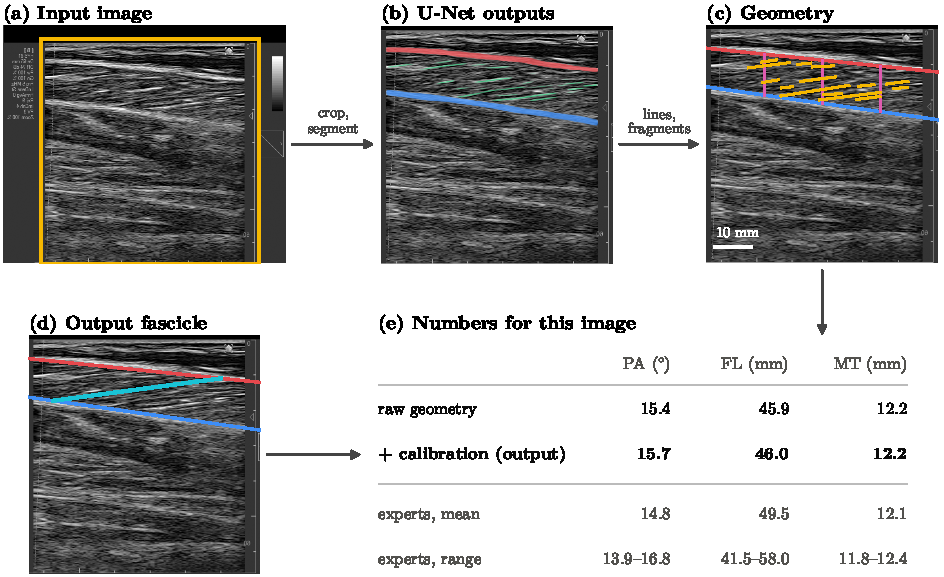
\includegraphics[width=\textwidth]{figures/fig1_pipeline.pdf}
\caption{One image through the pipeline. (a) Input image and ultrasound box (gold). (b) Network outputs: superficial (red) and deep (blue) aponeurosis, fascicle map (green). (c) Geometry on the 8\,px/mm grid: straight aponeurosis lines, MT at 25, 50 and 75\% of the width (pink), fascicle fragments used for PA (gold). (d) The output as a straight fascicle at the final PA (cyan). (e) Numbers at each stage, with leave-one-out calibration, against the seven expert raters. The image is im\_16 of the UMUD benchmark (CC BY 4.0), the one with the median leave-one-out score of the 35 images; its scale comes with the benchmark, and the learned correction of Section~\ref{sec:learned} is not applied to it. Competition images are not shown because the competition rules do not allow publishing them.}
\label{fig:pipeline}
\end{figure}

\subsection{Scale}

A ruler decoder, adapted from a public notebook by AmbrosM, recognises the six screen layouts and reads the vertical depth ruler to get px/cm and the box of the ultrasound image. On all 309 frames the decoded depth is a multiple of 0.5\,cm to within 1.2\,mm, which is how scanners set depth. On one Telemed layout (90 frames) the horizontal ticks give a scale 0.905 times the vertical one; following the hosts' statement that the raters used the vertical scale for both axes, we treat pixels as square.

\subsection{Segmentation}

We use U-Nets from \texttt{segmentation\_models\_pytorch} with ImageNet encoders, a one-channel grey input, BCE + Dice loss, AdamW (learning rate $3\cdot10^{-4}$), a one-cycle schedule, bf16, five folds grouped by near-duplicate frames of the same video, and horizontal-flip test-time augmentation. Augmentations: flip, rotation $\pm8^\circ$, zoom 0.85--1.2, horizontal stretch 0.9--1.1, gamma and gain, blur, multiplicative noise.

The aponeurosis network is a ConvNeXt-Tiny U-Net on the ultrasound box squeezed to $512\times512$, with two output channels (superficial, deep); validation Dice is 0.85 and 0.83. The fascicle map is the mean of three networks. One is the same square ConvNeXt-Tiny. The other two (ConvNeXt-Tiny, 5 folds; EfficientNet-B4, 3 folds) see the image with its aspect ratio kept: shorter side 512, random $512\times512$ crops in training, overlapping tiles at inference. Squeezing to a square changes angles: a $15^\circ$ fascicle appears at $12$--$19^\circ$ depending on the scanner. These two networks also predict the fascicle direction as $(\cos 2\theta, \sin 2\theta)$ per pixel, supervised by the direction of the mask lines; their Dice is 0.41--0.44 and the direction error about $5^\circ$.

The same aspect-preserving tiling made the aponeurosis network much worse: on tall images a tile often contains a single aponeurosis, and the network cannot tell whether it is the upper or the lower one.

\subsection{Geometry}

\paragraph{Aponeuroses.} Each aponeurosis is a straight line $y=ax+b$ fitted to the inner edge of its band (lower edge of the superficial, upper edge of the deep), refitted after dropping columns with residuals above $3\,\mathrm{median}+1$\,px. If the deep channel shows several bands, as when two muscles are stacked, we take the uppermost band with less than 15\% of the fascicle mass below it, since the raters measure the upper muscle.

\paragraph{MT} is the mean perpendicular distance between the lines at 25, 50 and 75\% of the width.

\paragraph{PA.} Connected components of the fascicle map ($p>0.5$) are fragments. For a fragment with pixel-covariance eigenvalues $\lambda_1\ge\lambda_0$ and principal direction $\theta$, the length is $\sqrt{12\lambda_1}$, since a uniform segment of length $L$ has variance $L^2/12$ along its axis. We keep fragments longer than 3\,mm with $\lambda_0\le0.1\lambda_1$, centred within 10--90\% of the width and 12--88\% of the depth between the aponeuroses. PA is the length-weighted median of the fragment angles to the deep aponeurosis.

\paragraph{FL.} There are two estimates: $\FL_\mathrm{trig}=\MT/\sin\PA$, and $\FL_\mathrm{line}$, the length of a straight line at the mean fascicle orientation from the centre of the deep aponeurosis to the superficial one. The output is $w\,\FL_\mathrm{line}+(1-w)\,\FL_\mathrm{trig}$ with $w=0.2$, chosen on the benchmark.

\subsection{Calibration on the benchmark}

For each target we choose among no correction, an offset $y=x+c$ and a scale $y=sx$ by leave-one-out MAE on the 35 benchmark images. The offset is the median of residuals, which minimises MAE. For the scale we use the median of ratios; the exact MAE minimiser is the median of $y_i/x_i$ weighted by $|x_i|$, a difference we did not test. On top of this, PA gets a manual offset so that the total shift is $+2.0^\circ$, chosen on the public leaderboard (Section~\ref{sec:lb-use}).

\subsection{Learned correction from manual test labels}
\label{sec:learned}

Kaggle's general rules forbid using hand labels of test records, but the competition host confirmed that manual measurements of the test images may train or calibrate an automated model if this is declared as external data (competition discussion 690868, on rule 3.4(b)). We declare that use here: our submissions from v5 onwards depend on these measurements, and they never reach the output directly. One team member, Arman Zhalgasbayev, measured all 309 frames in a browser tool: two points per aponeurosis and one fascicle per frame. We recompute PA, FL and MT from the points with our ruler scale and map them to the hosts' convention by $\PA+0.75^\circ$, $\FL\times1.04$, $\MT\times0.97$. This map was chosen so that score differences between eight of our submissions, computed against the labels, match their public leaderboard differences: over a grid of offsets and scales we minimised the mean absolute gap between centred local and centred leaderboard scores. The correlation after the map is 0.98, with three parameters fitted on eight points.

A gradient-boosting model then learns the residual of the geometry. About 40 features per frame describe what the networks found: length-weighted quantiles of fragment angles overall, near each aponeurosis, in the centre and at the edges; fragment counts and lengths; aponeurosis slopes and convergence; MT near the edges; raw PA, FL, MT; scale and layout. Targets are $\Delta\PA$, $\log(\FL_\mathrm{label}/\FL)$ and $\Delta\MT$, averaged within each 5-frame series, because frames of a series are nearly identical and their label spread (mean absolute deviation from the series median: PA $0.6^\circ$, FL 4.2\,mm, MT 0.15\,mm) is annotator noise. The model is scikit-learn's \texttt{HistGradientBoostingRegressor} with absolute-error loss, depth 3, 200 iterations, learning rate 0.05 and at least 15 samples per leaf. Predictions are cross-fitted: 5-fold GroupKFold by series, repeated with 5 seeds, so every frame is corrected by models that never saw its series. About 200 independent units remain after grouping.

\subsection{Post-processing}

We take the median within each 5-frame series and clip to the ranges in the data description (PA 5--45$^\circ$, FL 30--200\,mm, MT 10--50\,mm). The metric is an MAE, so medians are the right aggregate.

\subsection{What the leaderboard influenced}
\label{sec:lb-use}

Every value in our submissions is computed by code from the image. No value was set or edited by hand for any frame, and predictions of other teams or public notebooks were not blended in; one public prediction table served only to find frames worth inspecting. The manual measurements enter only as training targets of the cross-fitted model, so a frame is corrected by models that never saw its series. The pipeline runs on new images without a leaderboard, which is the host's criterion for a valid submission (competition discussion 739660).

The pipeline is not independent of the public leaderboard, though. Four constants and one choice come from it, and all five are frozen in the code:
\begin{itemize}
\item the PA offset, chosen by hand from three submissions (total shift $0^\circ$, $+2^\circ$, $+4^\circ$);
\item the three numbers of the convention map of Section~\ref{sec:learned}, found by a grid search over the public scores of eight submissions, which is the one automated step;
\item the final variant, the best public score among five candidates whose differences are within the leaderboard noise.
\end{itemize}
We also looked at test images during development: one test series prompted the rule for stacked muscles in Section~4.3. We made 18 submissions in total, including probes and the diagnostic one in Table~\ref{tab:results}, and stopped once the remaining gains looked like fitting the raters of this test set.

\section{Analysis}

\subsection{PA error drives the score through FL}
\label{sec:propagation}

With $\FL=h/\sin\alpha$ for thickness $h$ and angle $\alpha$,
\begin{equation}
\frac{\partial\,\FL}{\partial\alpha} = -\frac{h\cos\alpha}{\sin^2\alpha} = -\FL\cot\alpha .
\end{equation}
A PA error of $\delta$ degrees therefore costs $\FL\cot\alpha\cdot\pi\delta/180$\,mm of FL. In score units, the ratio of the FL term to the PA term is
\begin{equation}
\rho(\alpha) = \frac{\FL\cot\alpha\cdot\pi/180\,/\,12}{1/6} = \frac{\pi}{360}\,\FL\cot\alpha .
\end{equation}
PA error matters more through FL than directly whenever $\FL\cot\alpha > 360/\pi \approx 115$\,mm (Table~\ref{tab:sens}, Figure~\ref{fig:sens}). This covers most VL and RF images: 78\% of our test predictions have PA below $20^\circ$.

\begin{table}[t]
\centering\small
\caption{FL sensitivity to PA for typical geometries.}
\label{tab:sens}
\begin{tabular}{@{}rrrrr@{}}
\toprule
MT (mm) & PA ($^\circ$) & FL (mm) & $\partial\FL$ per $1^\circ$ PA (mm) & $\rho$ \\
\midrule
20 & 10 & 115 & 11.4 & 5.7 \\
22 & 12 & 106 & 8.7 & 4.3 \\
20 & 15 & 77 & 5.0 & 2.5 \\
20 & 25 & 47 & 1.8 & 0.9 \\
18 & 30 & 36 & 1.1 & 0.5 \\
\bottomrule
\end{tabular}
\end{table}

\begin{figure}[t]
\centering
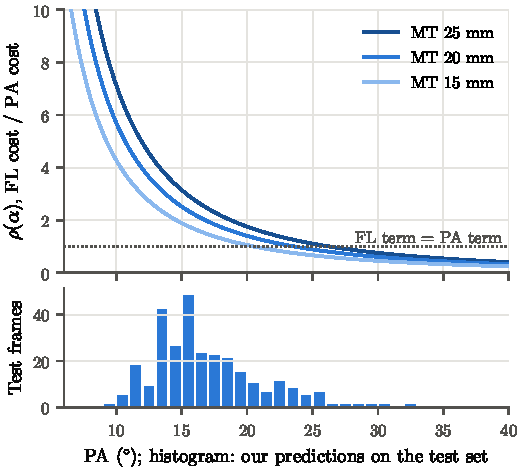
\includegraphics[width=0.6\textwidth]{figures/fig2_sensitivity.pdf}
\caption{Top: ratio $\rho(\alpha)$ of the FL term to the PA term of the score caused by the same PA error. Bottom: distribution of our PA predictions on the test set.}
\label{fig:sens}
\end{figure}

The test data agree (Figure~\ref{fig:errors}). Against the manual labels (all 309 frames), FL makes up 62\% of our score, PA 24\% and MT 14\%; per-frame errors in PA and FL correlate at $-0.81$; and a per-frame regression gives $S_i \approx 0.13 + 0.14\,|e_{\PA,i}|$. The score falls from 0.47 for frames with labelled PA below $12^\circ$ to 0.23 above $25^\circ$. If FL is measured as a straight centred fascicle between our aponeurosis lines (with one global scale of 1.13), its MAE is 7.7\,mm with our PA and 3.6\,mm with the labelled PA.

\begin{figure}[t]
\centering
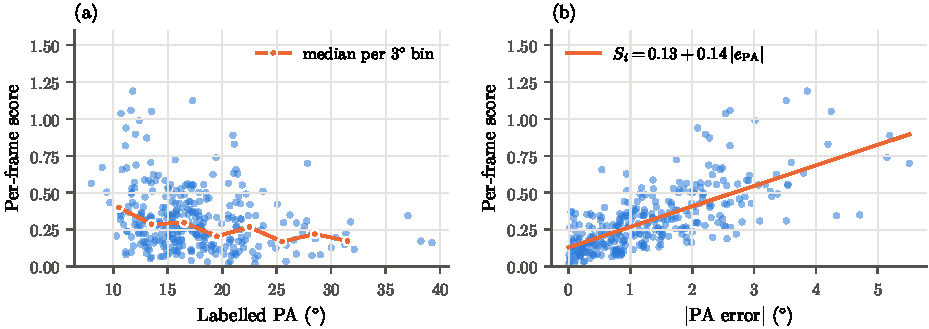
\includegraphics[width=\textwidth]{figures/fig3_errors.pdf}
\caption{Per-frame score of our final submission against the manual labels (309 test frames). (a) Against the labelled PA, with medians per $3^\circ$ bin (bins with at least 5 frames). (b) Against the absolute PA error, with a least-squares line.}
\label{fig:errors}
\end{figure}

\subsection{Non-parallel aponeuroses}

$\MT/\sin\PA$ assumes parallel aponeuroses. Let the superficial aponeurosis make an angle $\gamma$ with the deep one, and let a straight fascicle leave the deep aponeurosis at angle $\alpha$ at a point where the thickness is $h$. The fascicle and the two lines form a triangle, and the law of sines gives
\begin{equation}
L = \frac{h}{\sin(\alpha + s\gamma)},\qquad
s=\begin{cases}+1 & \text{fascicle runs towards the convergence,}\\ -1 & \text{otherwise.}\end{cases}
\end{equation}
To first order, $\MT/\sin\alpha$ has relative error $s\gamma\cot\alpha$: 16\% for $\alpha=12^\circ$, $\gamma=2^\circ$. The thickness at the fascicle's end also differs from the mean MT, which adds a second error of the same order. On the benchmark consensus the ratio $\FL/(\MT/\sin\PA)$ has median 1.07 and range 0.63--1.41, and the two differ by 6.5\,mm MAE. On the two test layouts with strongly converging aponeuroses (20 frames), $\MT/\sin\PA$ has an FL MAE of 15.5\,mm against the labels, and extending each fragment to both lines cuts it to 7.1\,mm. In the final pipeline the learned correction absorbs this effect.

\subsection{Orientation from raw ultrasound is biased towards horizontal}
\label{sec:speckle}

Before the first submission, our pipeline measured fascicle orientation with a coherence-weighted structure tensor on the raw image,
\begin{equation}
J = G_\sigma * (\nabla I\,\nabla I^\top),\qquad \hat\theta = \tfrac12\operatorname{atan2}(2J_{xy},\,J_{xx}-J_{yy}) + \tfrac{\pi}{2}.
\end{equation}
On the 35 benchmark images it underestimated PA on every image, by $5.6^\circ$ on average, and the bias grew with the true angle (correlation $-0.63$ between bias and expert PA; Figure~\ref{fig:speckle}). The same tensor on the fascicle probability map gives a bias of $-0.79^\circ$ and an MAE of $1.03^\circ$.

\begin{figure}[t]
\centering
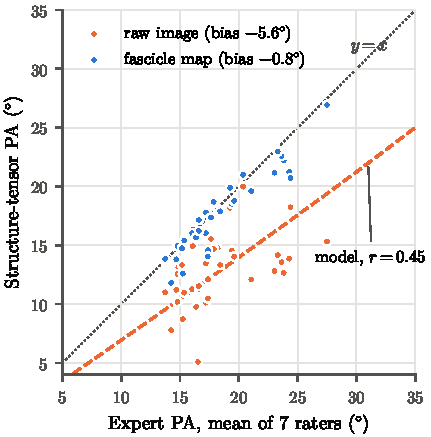
\includegraphics[width=0.55\textwidth]{figures/fig4_speckle.pdf}
\caption{Structure-tensor PA on the 35 UMUD benchmark images, computed on the raw image and on the fascicle probability map, against the mean of 7 expert raters. Dashed: the speckle mixing model (\ref{eq:mix}) with $r$ fitted to the raw-image estimates.}
\label{fig:speckle}
\end{figure}

A simple model explains the trend. Speckle in B-mode images is elongated laterally, since the lateral resolution of the beam is coarser than the axial one \citep{wagner1983speckle}, so speckle adds tensor energy with horizontal line orientation. In the doubled-angle representation, fascicles at angle $\alpha$ to the horizontal contribute $a(\cos2\alpha, \sin2\alpha)$ and speckle contributes $b(1,0)$. With $r=b/a$,
\begin{equation}
\tan 2\hat\alpha = \frac{\sin 2\alpha}{\cos 2\alpha + r}.
\label{eq:mix}
\end{equation}
The estimate is pulled towards zero, and the pull grows with $\alpha$: for $r=0.39$ the bias is $2.2^\circ$ at $8^\circ$, $4.2^\circ$ at $15^\circ$ and $5.5^\circ$ at $20^\circ$. Fitting the single parameter $r$ to the benchmark gives $r=0.45$ and reduces the MAE of raw-image PA from $5.6^\circ$ to $2.2^\circ$. We use the model only to explain the bias; the network map removes it without a correction. Against the manual test labels, after the best constant offset, a Gabor filter bank on the raw image reaches $1.90^\circ$ MAE and a Radon projection of the fascicle map $1.52^\circ$, against $1.37^\circ$ for fragment angles. Estimates that work on the fascicle map pixel by pixel, the structure tensor ($1.32^\circ$) and the direction head ($1.33^\circ$), are as good as fragments.

\subsection{Convention matters more than pixels}

On the benchmark, the final pipeline with leave-one-out calibration scores 0.204 against the 7-rater consensus and 0.239 against pairs of raters (mean over the 21 pairs), better than the best single rater against pairs of the others (0.29) and DL\_Track\_US (0.37). On the test set the picture is different. Our first submission, calibrated the same way, scored 0.563 on the public leaderboard. A global PA offset of $+2^\circ$ moved a later version from 0.529 to 0.480, and $+4^\circ$ gave 0.610. The same offset makes the final pipeline worse on the benchmark: 0.280 against the consensus and 0.299 against pairs.

The test raters therefore measure PA about $2^\circ$ steeper than the benchmark consensus, outside the range of individual benchmark biases ($-1.0^\circ$ to $+1.3^\circ$). The fragment angles suggest why. Taking the 50th, 75th or 90th length-weighted percentile of fragment angles per frame gives nearly the same MAE against the manual labels after the best offset ($1.33$--$1.37^\circ$), but the offsets differ: $+2.3^\circ$, $+1.2^\circ$ and $+0.1^\circ$. The raters seem to pick the steepest clear fascicles in the frame, which agrees with the hosts' description of choosing central fascicles that need the least extrapolation.

For the 20 Telemed series with the largest error (42\% of the total), we split the raw PA error (our fragment PA minus the annotator's PA) into three additive parts: the deep aponeurosis line (our fragments measured to our line and to the annotator's line), the choice of fascicles (all our fragments against the fragments lying along the annotator's fascicle) and the drawn line (those fragments against the annotator's line). Table~\ref{tab:decomp} gives each part's share of the between-series variance, computed as $\operatorname{cov}(\text{part},\text{total})/\operatorname{var}(\text{total})$ so that the shares add up to about one. The aponeurosis contributes little: our deep line differs from the annotator's by $0.3^\circ$ on average and $0.9^\circ$ at most. The largest part is the drawn line. Along the very fascicle the annotator measured, our fragments are $1.3^\circ$ flatter than the annotator's line (median over series), which is close to the $+2^\circ$ offset the test raters needed. Hand-drawn lines seem to run steeper than the texture they follow, and on some frames the line crosses two or three parallel fragments instead of following one. Which fascicle is chosen comes second.

\begin{table}[t]
\centering\small
\caption{Decomposition of the raw PA error on the 20 Telemed series with the largest error (97 frames), against the manual labels. Share is $\operatorname{cov}(\text{part},\text{total})/\operatorname{var}(\text{total})$ across series medians.}
\label{tab:decomp}
\begin{tabular}{@{}lrrr@{}}
\toprule
Part & Median ($^\circ$) & SD across series ($^\circ$) & Share \\
\midrule
deep aponeurosis line & $-0.1$ & 0.4 & 8\% \\
choice of fascicles & $-0.1$ & 1.2 & 39\% \\
drawn line along the chosen fascicle & $-1.3$ & 1.3 & 59\% \\
\bottomrule
\end{tabular}
\end{table}

\subsection{Labels from one non-expert: what transfers and what leaks}
\label{sec:leak}

The manual labels helped in one specific role. Used as targets for the cross-fitted residual model, they improved the public score from 0.441 to 0.385, mostly through FL (local MAE 8.9 to 7.3\,mm); PA hardly changed, since a correction cannot recover fascicles the network does not see.

Submitted as predictions after the convention map, the labels scored 0.458, worse than the model. A non-expert placing one fascicle per frame is a noisy rater: the within-series spread alone amounts to about 0.17 score units.

Components trained directly on the clicks misled local validation. We fine-tuned the aponeurosis network on the annotator's lines, cross-fitted by series: Dice of the deep aponeurosis on held-out test series rose from 0.62 to 0.75, and together with rotation TTA (which alone changed the local score by 0.002) the local score improved from 0.326 to 0.309, while the public score worsened from 0.385 to 0.395. A random public split explains a reversal of this size with a probability of about 0.3\% (20\,000 random thirds scored against the manual labels). Cross-fitting by series does not protect against this, because the annotator's style is shared by all series: the network learned where this person clicks. The residual model is less exposed because its features come from networks trained on the training set only, but its local score is still optimistic. Across the five later submissions (v5 to v9), local and public scores did not correlate (Pearson $-0.68$, public range 0.383--0.395, all within the leaderboard noise).

\subsection{Probing a small public leaderboard}
\label{sec:probing}

A public split of about 102 images limits what a leaderboard can tell. For pairs of our later submissions, the score difference on a random third of the test set has a standard deviation of 0.004--0.010 (against the manual labels), so differences below 0.02 were invisible to every check we had: public leaderboard, manual labels and benchmark.

Single-sided probes also mislead. Let $r$ be the residual of one target and $F$ its distribution function. Shifting all predictions by $c>0$ changes the MAE by
\begin{equation}
\Delta(c) = \mathbb{E}|r-c| - \mathbb{E}|r| = \int_0^c \bigl(2F(t)-1\bigr)\,dt = c\,\bigl(2F(0)-1\bigr) + 2\int_0^c \bigl(F(t)-F(0)\bigr)\,dt .
\end{equation}
The first term measures bias; the second is non-negative and close to $f(0)\,c^2$ for density $f$. A one-sided increase of the score can come entirely from the second term. We read MT $-0.75$\,mm (0.441 to 0.484) and FL $\times0.95$ (to 0.496) as evidence that both targets were too low; a fourth probe, MT and FL $\times1.04$, also made the score worse (0.505), so the base was near the optimum and the first reading was wrong. Paired probes separate the two terms:
\begin{equation}
2F(0)-1 \approx \frac{\Delta(c)-\Delta(-c)}{2c},\qquad f(0) \approx \frac{\Delta(c)+\Delta(-c)}{2c^2}.
\end{equation}
Section~\ref{sec:lb-use} lists what we took from the leaderboard.

\section{Results}

Table~\ref{tab:results} lists our submissions. Our last submission dates from 24 October 2026, when it ranked 95th of 482 on the public leaderboard. On 6 November it ranks 197th of 601 (top public score 0.166, 50th place 0.241). Private: \private.

By layout, the error concentrates on one Telemed layout (90 frames, score 0.42 against the labels, 38\% of the total error), where shallow angles amplify PA error into FL. The other layouts score 0.22--0.31.

\begin{table}[t]
\centering\small
\caption{Submissions in chronological order (2026). Local score is against the manual labels mapped to the hosts' convention; from v5 onwards it is cross-fitted.}
\label{tab:results}
\begin{tabular}{@{}lllrr@{}}
\toprule
Date & Version & Change & Local & Public \\
\midrule
16.10 & v1 & one fold, PA from structure tensor on the fascicle map & & 0.563 \\
17.10 & v2 & PA from fascicle fragments & 0.493 & 0.529 \\
17.10 & v2 $+2^\circ$ & global PA offset & 0.421 & 0.480 \\
17.10 & v3 & five folds, PA $+2^\circ$ & 0.414 & 0.441 \\
18.10 & v4 & deep aponeurosis chosen by fascicles & 0.378 & -- \\
23.10 & v5 & v4 + learned correction & 0.326 & 0.385 \\
23.10 & v7 & v5 + aponeurosis net fine-tuned on manual lines, rotation TTA & 0.309 & 0.395 \\
24.10 & v9a & unsqueezed ConvNeXt fascicle net instead of the square one & 0.314 & 0.391 \\
24.10 & v9, 2 nets & mean of square and unsqueezed ConvNeXt & 0.321 & 0.394 \\
24.10 & v9, 3 nets & mean of three fascicle nets (final) & 0.320 & \textbf{0.383} \\
24.10 & labels & manual labels as the answer (diagnostic only) & & 0.458 \\
\bottomrule
\end{tabular}
\end{table}

Several ideas did not help, each checked locally or with a submission: rotation test-time augmentation ($\pm4^\circ$); PA from a Radon projection, a Gabor bank or the direction head (Section~\ref{sec:speckle}); PA to a local quadratic tangent of the deep aponeurosis instead of a straight line (worse on the benchmark and against the labels); intensity normalisation with depth; a 768\,px fascicle network; fragment thresholds 0.3--0.4; FL recomputed from the corrected PA instead of a separate FL correction.

\section{Limitations}

The benchmark has 35 images and seven raters. The competition host is one of them (competition discussion 739660), but the test labels come from two researchers, so the benchmark convention need not be the test convention. The manual labels come from one non-expert with one fascicle per frame, and the convention map was fitted on eight leaderboard scores and did not hold up out of sample (Section~\ref{sec:leak}). Most local numbers in Section~5 use these labels as the reference, so they describe agreement with the labels, not with the hosts. The aponeurosis network sees a square, angle-distorting input; we measure after mapping back. The ruler decoder knows only the six test layouts.

\section{Conclusions}

For segmentation-plus-geometry pipelines on muscle ultrasound, three things set the error: how raters choose and draw fascicles, how PA error propagates into FL at shallow angles, and whether the orientation estimate is biased by speckle. Segmentation quality beyond a moderate level mattered little in our experiments; new encoders, larger inputs and extra fascicle networks changed the public score by less than its noise. For future measurement benchmarks, publishing per-rater measurements, the lines each rater drew and the reconciliation rule would let methods target a convention explicitly instead of learning it from a leaderboard.

\section*{Code and data availability}

Code: \url{https://github.com/Aldabergenov1/umud-challenge} under GPL-3.0. With the trained weights, the notebook reruns the final submission in about 7 minutes on one GPU; the rerun differs from the submitted file only by the nondeterminism of GPU inference (mean differences $0.06^\circ$ PA, 0.4\,mm FL, 0.02\,mm MT) and gives the same local score. Competition data: CC BY-NC-SA 4.0, available to participants on Kaggle and not redistributed here. UMUD benchmark: CC BY 4.0, \url{https://osf.io/xbawc}. The manual test measurements are in the repository as point coordinates, without images, under CC BY-NC-SA 4.0. We used anonymised images provided by the organisers and the public UMUD benchmark, and collected no new data from participants.

\bibliographystyle{plainnat}
\bibliography{refs}

\end{document}
